%% bare_jrnl.tex
%% V1.4b
%% 2015/08/26
%% by Michael Shell
%% see http://www.michaelshell.org/
%% for current contact information.
%%
%% This is a skeleton file demonstrating the use of IEEEtran.cls
%% (requires IEEEtran.cls version 1.8b or later) with an IEEE
%% journal paper.
%%
%% Support sites:
%% http://www.michaelshell.org/tex/ieeetran/
%% http://www.ctan.org/pkg/ieeetran
%% and
%% http://www.ieee.org/

%%*************************************************************************
%% Legal Notice:
%% This code is offered as-is without any warranty either expressed or
%% implied; without even the implied warranty of MERCHANTABILITY or
%% FITNESS FOR A PARTICULAR PURPOSE! 
%% User assumes all risk.
%% In no event shall the IEEE or any contributor to this code be liable for
%% any damages or losses, including, but not limited to, incidental,
%% consequential, or any other damages, resulting from the use or misuse
%% of any information contained here.
%%
%% All comments are the opinions of their respective authors and are not
%% necessarily endorsed by the IEEE.
%%
%% This work is distributed under the LaTeX Project Public License (LPPL)
%% ( http://www.latex-project.org/ ) version 1.3, and may be freely used,
%% distributed and modified. A copy of the LPPL, version 1.3, is included
%% in the base LaTeX documentation of all distributions of LaTeX released
%% 2003/12/01 or later.
%% Retain all contribution notices and credits.
%% ** Modified files should be clearly indicated as such, including  **
%% ** renaming them and changing author support contact information. **
%%*************************************************************************


% *** Authors should verify (and, if needed, correct) their LaTeX system  ***
% *** with the testflow diagnostic prior to trusting their LaTeX platform ***
% *** with production work. The IEEE's font choices and paper sizes can   ***
% *** trigger bugs that do not appear when using other class files.       ***                          ***
% The testflow support page is at:
% http://www.michaelshell.org/tex/testflow/



\documentclass[journal]{IEEEtran}
\usepackage[usenames]{color}
\usepackage{epsfig}
\usepackage{graphics}
\usepackage{caption}
\usepackage{amsmath}
\usepackage{amssymb}
\usepackage{multirow}
\usepackage{cite}
\usepackage{array}
\usepackage{pslatex} 
\usepackage{url}
\usepackage{lineno}
\usepackage{graphicx}  % Written by David Carlisle and Sebastian Rahtz
\usepackage{setspace}
\usepackage{tikz}
\usepackage{hhline}
\usepackage{mathtools}
\usepackage{caption}
\usepackage[letterpaper]{geometry}
\geometry{verbose,tmargin=0.7in,bmargin=0.7in,lmargin=0.65in,rmargin=0.65in}
\setlength{\headheight}{17pt}
\setlength{\headsep}{5pt}
 \newcommand{\flogo}{
\includegraphics[height=18pt]{Logo.jpg}
 }
%\captionsetup{labelfont={up},font=small}
\captionsetup[figure]{name={Fig.},labelsep=period,font=small}
 \captionsetup[table]{name={TABLE},labelsep=period,font=small}
% If IEEEtran.cls has not been installed into the LaTeX system files,
% manually specify the path to it like:
% \documentclass[journal]{../sty/IEEEtran}




% Some very useful LaTeX packages include:
% (uncomment the ones you want to load)


% *** MISC UTILITY PACKAGES ***
%
\usepackage{ifpdf}
% Heiko Oberdiek's ifpdf.sty is very useful if you need conditional
% compilation based on whether the output is pdf or dvi.
% usage:
% \ifpdf
%   % pdf code
% \else
%   % dvi code
% \fi
% The latest version of ifpdf.sty can be obtained from:
% http://www.ctan.org/pkg/ifpdf
% Also, note that IEEEtran.cls V1.7 and later provides a builtin
% \ifCLASSINFOpdf conditional that works the same way.
% When switching from latex to pdflatex and vice-versa, the compiler may
% have to be run twice to clear warning/error messages.






% *** CITATION PACKAGES ***
%
\usepackage{cite}
% cite.sty was written by Donald Arseneau
% V1.6 and later of IEEEtran pre-defines the format of the cite.sty package
% \cite{} output to follow that of the IEEE. Loading the cite package will
% result in citation numbers being automatically sorted and properly
% "compressed/ranged". e.g., [1], [9], [2], [7], [5], [6] without using
% cite.sty will become [1], [2], [5]--[7], [9] using cite.sty. cite.sty's
% \cite will automatically add leading space, if needed. Use cite.sty's
% noadjust option (cite.sty V3.8 and later) if you want to turn this off
% such as if a citation ever needs to be enclosed in parenthesis.
% cite.sty is already installed on most LaTeX systems. Be sure and use
% version 5.0 (2009-03-20) and later if using hyperref.sty.
% The latest version can be obtained at:
% http://www.ctan.org/pkg/cite
% The documentation is contained in the cite.sty file itself.






% *** GRAPHICS RELATED PACKAGES ***
%
\ifCLASSINFOpdf
  \usepackage{graphicx}
  % declare the path(s) where your graphic files are
  \graphicspath{{gfx}}
  % and their extensions so you won't have to specify these with
  % every instance of \includegraphics
  \DeclareGraphicsExtensions{.pdf,.jpeg,.png,.eps}
\else
  % or other class option (dvipsone, dvipdf, if not using dvips). graphicx
  % will default to the driver specified in the system graphics.cfg if no
  % driver is specified.
  % \usepackage[dvips]{graphicx}
  % declare the path(s) where your graphic files are
  % \graphicspath{{../eps/}}
  % and their extensions so you won't have to specify these with
  % every instance of \includegraphics
  % \DeclareGraphicsExtensions{.eps}
\fi
% graphicx was written by David Carlisle and Sebastian Rahtz. It is
% required if you want graphics, photos, etc. graphicx.sty is already
% installed on most LaTeX systems. The latest version and documentation
% can be obtained at: 
% http://www.ctan.org/pkg/graphicx
% Another good source of documentation is "Using Imported Graphics in
% LaTeX2e" by Keith Reckdahl which can be found at:
% http://www.ctan.org/pkg/epslatex
%
% latex, and pdflatex in dvi mode, support graphics in encapsulated
% postscript (.eps) format. pdflatex in pdf mode supports graphics
% in .pdf, .jpeg, .png and .mps (metapost) formats. Users should ensure
% that all non-photo figures use a vector format (.eps, .pdf, .mps) and
% not a bitmapped formats (.jpeg, .png). The IEEE frowns on bitmapped formats
% which can result in "jaggedy"/blurry rendering of lines and letters as
% well as large increases in file sizes.
%
% You can find documentation about the pdfTeX application at:
% http://www.tug.org/applications/pdftex





% *** MATH PACKAGES ***
%
\usepackage{amsmath}
% A popular package from the American Mathematical Society that provides
% many useful and powerful commands for dealing with mathematics.
%
% Note that the amsmath package sets \interdisplaylinepenalty to 10000
% thus preventing page breaks from occurring within multiline equations. Use:
\interdisplaylinepenalty=2500
% after loading amsmath to restore such page breaks as IEEEtran.cls normally
% does. amsmath.sty is already installed on most LaTeX systems. The latest
% version and documentation can be obtained at:
% http://www.ctan.org/pkg/amsmath





% *** SPECIALIZED LIST PACKAGES ***
%
\usepackage{algorithmic}
% algorithmic.sty was written by Peter Williams and Rogerio Brito.
% This package provides an algorithmic environment fo describing algorithms.
% You can use the algorithmic environment in-text or within a figure
% environment to provide for a floating algorithm. Do NOT use the algorithm
% floating environment provided by algorithm.sty (by the same authors) or
% algorithm2e.sty (by Christophe Fiorio) as the IEEE does not use dedicated
% algorithm float types and packages that provide these will not provide
% correct IEEE style captions. The latest version and documentation of
% algorithmic.sty can be obtained at:
% http://www.ctan.org/pkg/algorithms
% Also of interest may be the (relatively newer and more customizable)
% algorithmicx.sty package by Szasz Janos:
% http://www.ctan.org/pkg/algorithmicx




% *** ALIGNMENT PACKAGES ***
%
\usepackage{array}
% Frank Mittelbach's and David Carlisle's array.sty patches and improves
% the standard LaTeX2e array and tabular environments to provide better
% appearance and additional user controls. As the default LaTeX2e table
% generation code is lacking to the point of almost being broken with
% respect to the quality of the end results, all users are strongly
% advised to use an enhanced (at the very least that provided by array.sty)
% set of table tools. array.sty is already installed on most systems. The
% latest version and documentation can be obtained at:
% http://www.ctan.org/pkg/array


% IEEEtran contains the IEEEeqnarray family of commands that can be used to
% generate multiline equations as well as matrices, tables, etc., of high
% quality.




% *** SUBFIGURE PACKAGES ***
%\ifCLASSOPTIONcompsoc
%  \usepackage[caption=false,font=normalsize,labelfont=sf,textfont=sf]{subfig}
%\else
%  \usepackage[caption=false,font=footnotesize]{subfig}
%\fi
% subfig.sty, written by Steven Douglas Cochran, is the modern replacement
% for subfigure.sty, the latter of which is no longer maintained and is
% incompatible with some LaTeX packages including fixltx2e. However,
% subfig.sty requires and automatically loads Axel Sommerfeldt's caption.sty
% which will override IEEEtran.cls' handling of captions and this will result
% in non-IEEE style figure/table captions. To prevent this problem, be sure
% and invoke subfig.sty's "caption=false" package option (available since
% subfig.sty version 1.3, 2005/06/28) as this is will preserve IEEEtran.cls
% handling of captions.
% Note that the Computer Society format requires a larger sans serif font
% than the serif footnote size font used in traditional IEEE formatting
% and thus the need to invoke different subfig.sty package options depending
% on whether compsoc mode has been enabled.
%
% The latest version and documentation of subfig.sty can be obtained at:
% http://www.ctan.org/pkg/subfig




% *** FLOAT PACKAGES ***
%
%\usepackage{fixltx2e}
% fixltx2e, the successor to the earlier fix2col.sty, was written by
% Frank Mittelbach and David Carlisle. This package corrects a few problems
% in the LaTeX2e kernel, the most notable of which is that in current
% LaTeX2e releases, the ordering of single and double column floats is not
% guaranteed to be preserved. Thus, an unpatched LaTeX2e can allow a
% single column figure to be placed prior to an earlier double column
% figure.
% Be aware that LaTeX2e kernels dated 2015 and later have fixltx2e.sty's
% corrections already built into the system in which case a warning will
% be issued if an attempt is made to load fixltx2e.sty as it is no longer
% needed.
% The latest version and documentation can be found at:
% http://www.ctan.org/pkg/fixltx2e


%\usepackage{stfloats}
% stfloats.sty was written by Sigitas Tolusis. This package gives LaTeX2e
% the ability to do double column floats at the bottom of the page as well
% as the top. (e.g., "\begin{figure*}[!b]" is not normally possible in
% LaTeX2e). It also provides a command:
%\fnbelowfloat
% to enable the placement of footnotes below bottom floats (the standard
% LaTeX2e kernel puts them above bottom floats). This is an invasive package
% which rewrites many portions of the LaTeX2e float routines. It may not work
% with other packages that modify the LaTeX2e float routines. The latest
% version and documentation can be obtained at:
% http://www.ctan.org/pkg/stfloats
% Do not use the stfloats baselinefloat ability as the IEEE does not allow
% \baselineskip to stretch. Authors submitting work to the IEEE should note
% that the IEEE rarely uses double column equations and that authors should try
% to avoid such use. Do not be tempted to use the cuted.sty or midfloat.sty
% packages (also by Sigitas Tolusis) as the IEEE does not format its papers in
% such ways.
% Do not attempt to use stfloats with fixltx2e as they are incompatible.
% Instead, use Morten Hogholm'a dblfloatfix which combines the features
% of both fixltx2e and stfloats:
%
% \usepackage{dblfloatfix}
% The latest version can be found at:
% http://www.ctan.org/pkg/dblfloatfix




%\ifCLASSOPTIONcaptionsoff
%  \usepackage[nomarkers]{endfloat}
% \let\MYoriglatexcaption\caption
% \renewcommand{\caption}[2][\relax]{\MYoriglatexcaption[#2]{#2}}
%\fi
% endfloat.sty was written by James Darrell McCauley, Jeff Goldberg and 
% Axel Sommerfeldt. This package may be useful when used in conjunction with 
% IEEEtran.cls'  captionsoff option. Some IEEE journals/societies require that
% submissions have lists of figures/tables at the end of the paper and that
% figures/tables without any captions are placed on a page by themselves at
% the end of the document. If needed, the draftcls IEEEtran class option or
% \CLASSINPUTbaselinestretch interface can be used to increase the line
% spacing as well. Be sure and use the nomarkers option of endfloat to
% prevent endfloat from "marking" where the figures would have been placed
% in the text. The two hack lines of code above are a slight modification of
% that suggested by in the endfloat docs (section 8.4.1) to ensure that
% the full captions always appear in the list of figures/tables - even if
% the user used the short optional argument of \caption[]{}.
% IEEE papers do not typically make use of \caption[]'s optional argument,
% so this should not be an issue. A similar trick can be used to disable
% captions of packages such as subfig.sty that lack options to turn off
% the subcaptions:
% For subfig.sty:
% \let\MYorigsubfloat\subfloat
% \renewcommand{\subfloat}[2][\relax]{\MYorigsubfloat[]{#2}}
% However, the above trick will not work if both optional arguments of
% the \subfloat command are used. Furthermore, there needs to be a
% description of each subfigure *somewhere* and endfloat does not add
% subfigure captions to its list of figures. Thus, the best approach is to
% avoid the use of subfigure captions (many IEEE journals avoid them anyway)
% and instead reference/explain all the subfigures within the main caption.
% The latest version of endfloat.sty and its documentation can obtained at:
% http://www.ctan.org/pkg/endfloat
%
% The IEEEtran \ifCLASSOPTIONcaptionsoff conditional can also be used
% later in the document, say, to conditionally put the References on a 
% page by themselves.




% *** PDF, URL AND HYPERLINK PACKAGES ***
%
\usepackage{url}
% url.sty was written by Donald Arseneau. It provides better support for
% handling and breaking URLs. url.sty is already installed on most LaTeX
% systems. The latest version and documentation can be obtained at:
% http://www.ctan.org/pkg/url
% Basically, \url{my_url_here}.




% *** Do not adjust lengths that control margins, column widths, etc. ***
% *** Do not use packages that alter fonts (such as pslatex).         ***
% There should be no need to do such things with IEEEtran.cls V1.6 and later.
% (Unless specifically asked to do so by the journal or conference you plan
% to submit to, of course. )

% *** Custom ***
% \usepackage[utf8]{inputenc}
% \usepackage[backend=biber, style=ieee]{biblatex}
% \addbibresource{mybib.bib}
% \usepackage{csquotes}
\usepackage{soul}
\newcommand{\etal}{\textit{et al}., }
\newcommand{\ie}{\textit{i}.\textit{e}., }
\newcommand{\eg}{\textit{e}.\textit{g}.\ }
\newcommand{\cf}{\textit{cf}.\ }
\usepackage{hyperref}
\usepackage{siunitx}
\sisetup{parse-numbers = false}

% correct bad hyphenation here
\hyphenation{com-press-ive sens-ing cor-rel-a-tion}
\pagenumbering{gobble} 
 
% The paper headers
\usepackage[english]{babel}
\usepackage[utf8]{inputenc}
\usepackage{fancyhdr}
\pagestyle{fancy}
\fancyhf{}
\lhead{\flogo}
\fancyhead[L,RO]{\hl{PAPER ID NUMBER}}
\rhead{\textcolor{violet}{\Large\textbf{Technology Letter         }} \thepage}
\pagestyle{fancyplain}

\begin{document}
%
% paper title
% Titles are generally capitalized except for words such as a, an, and, as,
% at, but, by, for, in, nor, of, on, or, the, to and up, which are usually
% not capitalized unless they are the first or last word of the title.
% Linebreaks \\ can be used within to get better formatting as desired.
% Do not put math or special symbols in the title.
\title{\textcolor{violet}{Reverse Correlation Uncovers More Complete Tinnitus Spectra \vspace{0.25cm}}}

%
%
% author names and IEEE memberships
% note positions of commas and nonbreaking spaces ( ~ ) LaTeX will not break
% a structure at a ~ so this keeps an author's name from being broken across
% two lines.
% use \thanks{} to gain access to the first footnote area
% a separate \thanks must be used for each paragraph as LaTeX2e's \thanks
% was not built to handle multiple paragraphs
%

% \author{Alec Hoyland, %,~\IEEEmembership{Fellow, IEEE,}
%         Samantha Peznola, and Adam C. Lammert% <-this % stops a space
% \thanks{Paper submitted on DATE.
% 	This work was supported in part by the University of Massachusetts
% 	Center for Clinical and Translational Science Pilot Project Program 2022,
% 	grant number GRANT_NUMBER.
% 	Alec Hoyland is a graduate student in the Department of Biomedical Engineering
% 	at Worcester Polytechnic Institute (WPI), Worcester, MA, USA;
% 	Samantha Peznola is a Research Assistant at WPI;
% 	and Dr. Adam C. Lammert is Assistant Professor of Biomedical Engineering at WPI.
% }}
\author{Alec Hoyland, Nelson Barnett, Benjamin W. Roop, Adam C. Lammert\textsuperscript{\textdagger{}}%
\thanks{This work was supported in part by the University of Massachusetts
Center for Clinical and Translation Science Pilot Project Program 2022,
grant no. \hl{GRANT NUMBER}.}%
\thanks{Mr. Hoyland is a graduate student in the Department of Biomedical Engineering
at Worcester Polytechnic Institute (WPI) and a research scientist at Clarifai Inc.
Mr. Nelson Barnett is a research assistant at WPI.
Mr. Benjamin W. Roop is a research scientist at MIT Lincoln Laboratory.
Dr. Lammert is an Assistant Professor in the Department of Biomedical Engineering at WPI.}%
The authors declare no competing interests.
\thanks{\textsuperscript{\textdagger{}} Corresponding Author}%
\thanks{Code is freely available at \protect\url{https://github.com/alec-hoyland/tinnitus-project/}.
Data are available upon request.}}

% note the % following the last \IEEEmembership and also \thanks - 
% these prevent an unwanted space from occurring between the last author name
% and the end of the author line. i.e., if you had this:
% 
% \author{....lastname \thanks{...} \thanks{...} }
%                     ^------------^------------^----Do not want these spaces!
%
% a space would be appended to the last name and could cause every name on that
% line to be shifted left slightly. This is one of those "LaTeX things". For
% instance, "\textbf{A} \textbf{B}" will typeset as "A B" not "AB". To get
% "AB" then you have to do: "\textbf{A}\textbf{B}"
% \thanks is no different in this regard, so shield the last } of each \thanks
% that ends a line with a % and do not let a space in before the next \thanks.
% Spaces after \IEEEmembership other than the last one are OK (and needed) as
% you are supposed to have spaces between the names. For what it is worth,
% this is a minor point as most people would not even notice if the said evil
% space somehow managed to creep in.



% The paper headers
%\markboth{Journal of \LaTeX\ Class Files,~Vol.~14, No.~8, August~2015}%
%{Shell \MakeLowercase{\textit{et al.}}: Bare Demo of IEEEtran.cls for IEEE Journals}
% The only time the second header will appear is for the odd numbered pages
% after the title page when using the twoside option.
% 
% *** Note that you probably will NOT want to include the author's ***
% *** name in the headers of peer review papers.                   ***
% You can use \ifCLASSOPTIONpeerreview for conditional compilation here if
% you desire.




% If you want to put a publisher's ID mark on the page you can do it like
% this:
%\IEEEpubid{0000--0000/00\$00.00~\copyright~2015 IEEE}
% Remember, if you use this you must call \IEEEpubidadjcol in the second
% column for its text to clear the IEEEpubid mark.



% use for special paper notices
%\IEEEspecialpapernotice{(Invited Paper)}




% make the title area
\maketitle\thispagestyle{fancy}

% As a general rule, do not put math, special symbols or citations
% in the abstract or keywords.
\begin{abstract}
— \textit{Goal}: Make tinnitus characterization better.
\textit{Methods}: Use reverse correlation and compressed sensing.
\textit{Results}: Cool and fun results! Much data, very wow!
\textit{Conclusions}: Alec and Adam are cool and smart.
% The purpose of this document is to illustrate how one should prepare manuscripts for submission to the IEEE Open Journal of Engineering in Medicine and Biology (OJEMB). Please notice that this is the template for TECHNOLOGY LETTERS. These are short manuscripts with primary focus on the development of new devices, methods, and technologies. The material must be organized in a main manuscript body and a section entitled Supplementary Materials. The main manuscript body should be limited to 1,000 words and the material should be organized in the following sections (in the order shown here): Introduction, Materials and Methods, Results, Discussion, Conclusions. Authors can include in the main manuscript body up to 3 display items (i.e. figures and tables). In addition, the main manuscript body should include an abstract and up to 20 references. The references are not considered in the 1,000-word count. The abstract should be organized in subsections as shown here (i.e., Goal, Methods, Results, Conclusions). An impact statement should be included. The impact statement should be a short paragraph of no more than 30 words. Additional material should be included in the Supplementary Materials section of the manuscript. The Supplementary Materials section should either be organized in sections as per the main manuscript body (using up to 4,000 words) or it should be used to provide readers with a set of up to 10 additional display items (i.e. figures and tables). \textit{Methods}: Use this document as a template if you are using Latex. Otherwise, use this document as an instruction set. \textit{Results}: Paper titles should be written in uppercase and lowercase letters as shown above. Do not cite references in the abstract. Do not delete the blank line immediately above the abstract; it sets the footnote at the bottom of this column. The abstract should not exceed 150 words. \textit{Conclusions}: Preparing carefully your manuscript will lead to enhanced readability.
\end{abstract}

% Note that keywords are not normally used for peerreview papers.
\begin{IEEEkeywords}
    reverse correlation, tinnitus
\end{IEEEkeywords}

% For peer review papers, you can put extra information on the cover
% page as needed:
\ifCLASSOPTIONpeerreview
\begin{center} \bfseries EDICS Category: 3-BBND \end{center}
\fi
%
% For peerreview papers, this IEEEtran command inserts a page break and
% creates the second title. It will be ignored for other modes.
\IEEEpeerreviewmaketitle

\begin{minipage}[t]{1\columnwidth}
\textbf{\textit{Impact Statement}\textemdash{}\hl{30 words on significance}}\\
\\
\end{minipage}

\section{Introduction}

\IEEEPARstart{T}{INNITUS}\textemdash{}the perception of sound (\eg ringing, buzzing)
in the absence of an external stimulus\textemdash{}affects over 25 million people in the U.S.,
with some estimates ranged up to 50 million,
a third of which experience functional cognitive impairment and substantial reduction
in quality of life \cite{henryTinnitusEpidemiologicPerspective2020,vajsakovicPrinciplesMethodsPsychoacoustic2021}.
Primary treatment options for tinnitus are currently limited by a lack of methods
for accurately characterizing the internal sounds experienced by patients.
Tinnitus treatment typically involves \textit{sound therapy}, a form of habituation therapy,
which involves target exposure to external sounds to attenuate the perception of tinnitus
or to encourage patients to perceive their tinnitus as a neutral stimulus
\cite{jastreboff25YearsTinnitus2015}.
Critically, treatment outcomes have been repeatedly shown to improve
when the external sounds used in sound therapy are closely informed
by the internal tinnitus experience of the patient
\cite{steinInhibitioninducedPlasticityTinnitus2015,tassCounteractingTinnitusAcoustic2012,okamotoListeningTailormadeNotched2010,davisNeuromonicsTinnitusTreatment2007},
specifically, its component frequencies that constitute
the \textit{psychoacoustic tinnitus spectrum} (PTS).
However, existing methods for characterizing the PTS rely on reductionist assumptions
concerning the nature of tinnitus sounds (\eg that they are pure tones or have small-width Gaussian spectra)
and produce characterizations that are correspondingly bias and incomplete
when compared to the spectral variety of tinnitus percepts\textemdash{}less than
50\% of tinnitus patients
report their tinnitus sounding like ``ringing'' \cite{vajsakovicPrinciplesMethodsPsychoacoustic2021}.
There is a pressing need for methods to more completely characterize the PTS
\cite{henryTinnitusEpidemiologicPerspective2020,henryMeasurementTinnitus2016,norenaPsychoacousticCharacterizationTinnitus2002},
to further improve treatment outcomes for patients suffering from tinnitus.

We utilize \textit{reverse correlation} approach to characterize the PTS more completely,
without the strong biases introduced by existing methods.
Reverse correlation is a widely-accepted method for unconstrained and unbiased estimation
of latent neural representations (\eg neural receptive fields)
based on the white-noise method for black-box system identification
\cite{ringachReverseCorrelationNeurophysiology2004,ljungMeasureLackFit1978}.
This method has been used to characterize the psychophysical processes of perception
in vision (\eg faces) and audition (\eg phonemes)
\cite{ahumadaStimulusFeaturesSignal1971,gosselinSuperstitiousPerceptionsReveal2003,brimijoinInternalRepresentationVowel2013}
all on the basis of stimulus-response data
\cite{marmarelisWhiteNoiseMethodSystem1978,neriReceptivePerceptiveFields2006}.
In reverse correlation, subjects are presented with richly-varying random stimuli (\eg white noise)
and make simple ``yes/no'' responses about whether they perceive a particular signal
(\eg their tinnitus percept).
Internal representations, such as the PTS, can be estimated
by regressing subject responses against the stimuli over many trials.
Despite widespread use in characterizing neural and cognitive representations,
reverse correlation has never been used for tinnitus characterization.
% One limitation of reverse correlation is the sheer number of trials
% required to recover a good signal reconstruction.
% Classically, reverse correlation has required a large number of stimulus-response trials
% to yield accurate results (\eg 20,000 trials in \cite{gosselinSuperstitiousPerceptionsReveal2003}),
% a property that makes reverse correlation time-consuming in a clinical setting.

% We overcome this limitation of reverse correlation using \textit{compressed sensing} (CS)
% to reconstruct the PTS with high fidelity using far fewer trials.
% Compressive sensing can reduce the number of trials
% required an order of magnitude compared to conventional estimation, thereby allowing for efficient and
% accurate characterization of tinnitus within a single clinical visit. Compressive sensing has gained broad
% recognition in medical imaging \hl{[CITE]}, due to its ability to reduce scan times without sacrificing image quality or
% introducing bias, and its promise for similarly improving reverse correlation has been recently demonstrated by
% our group \textit{in-silico} \hl{[CITE]}.

In the present study, we validate a reverse correlation-based PTS reconstruction assay
on healthy hearing subjects via a template-matching experiment,
in which subjects compare the reverse correlation stimuli to a target tinnitus sample sound.
We benchmark the accuracy and reliability of the reconstructions,
using the target tinnitus signal as a ground truth.
High accuracy and reliablity measures relative to low numbers of trials per subject
provide evidence for the feasibility of the reverse correlation paradigm for uncovering
spectral representations of tinnitus.

Our long-term goal is to improve outcomes for patients suffering from tinnitus by providing a validated
clinical assay, based on the demonstrated capabilities of the reverse correlation approach, that clinicians can
use to accurately and efficiently characterize the individualized perceptual experience of tinnitus. Our guiding
hypothesis is that reverse correlation will produce PTS estimates that patients will consistently report as being
similar to their own tinnitus experience. The rationale for this work is that accurate and efficient characterization
of the PTS can inform individualized tinnitus treatment with enhanced habituation therapies.

% document is a Latex  template for Technology Letters to be submitted to IEEE OJEMB \cite{ahumadaStimulusFeaturesSignal1971}. Submissions must have the sections listed in the following exactly in the order shown here: Introduction, Materials and Methods, Results, Discussion, Conclusions. Manuscripts to be submitted to IEEE OJEMB as a Science Letters must use a different template. For both types of manuscript, the authors can opt to add a Supplementary Materials section.

% The very first letter is a 2 line initial drop letter followed
% by the rest of the first word in caps.
% 
% form to use if the first word consists of a single letter:
% \IEEEPARstart{A}{demo} file is ....
% 
% form to use if you need the single drop letter followed by
% normal text (unknown if ever used by the IEEE):
% \IEEEPARstart{A}{}demo file is ....
% 
% Some journals put the first two words in caps:
% \IEEEPARstart{T}{his demo} file is ....
% 
% Here we have the typical use of a "T" for an initial drop letter
% and "HIS" in caps to complete the first word.
% You must have at least 2 lines in the paragraph with the drop letter
% (should never be an issue)


\section{Materials and Methods }
% To use this template, type over sections of the template or cut and paste from another document. Highlight a section that you want to designate with a certain style, then select the appropriate name on the style menu. The style will adjust your fonts and line spacing. Do not change the font sizes or line spacing to squeeze more text into a limited number of pages. Use italics for emphasis; do not underline. 
% IEEE will do the final formatting of your paper. However, you should format your manuscript for submission to IEEE OJEMB for review and also for preparing for preprint that will be e-published several days after you upload the final version of an accepted manuscript. 

Software code used for the experiments and analysis was written in MATLAB (Mathworks, Inc., Natick, Massachusetts)
and is freely available at \protect\url{https://github.com/alec-hoyland/tinnitus-project/}.
The code depends on \cite{bechtoldViolinPlotsMatlab2022,kochYaml2022,gorur-shandilyaSrinivasGsMtools2022}.

\subsection{Stimulus Generation}

To generate stimuli, we partition the frequency space $f \in [100,~13,000]$ Hz
into $b=8$ mel-spaced frequency bins
so that each bin is perceptually different to a listener \cite{polfremanSoundSpottingFrameBased2001}
(\cf Supplementary Information).
All frequencies in the same bin have the same amplitude.
For each stimulus, we randomly select $[2,7]$ bins
with equal probability to be ``filled'' with power $0$ dB.
Unfilled bins are set to $-100$ dB.
The inverse Fourier transform of the spectrum yields a $500$-ms stimulus waveform.

% Before arriving at this method, we ran an \textit{in-silico} hyperparameter sweep over
% nine stimulus generation methods and hundreds of hyperparameter values
% (\cf Supplementary Information).

\subsection{Reconstruction Analysis}

A subject performing $n$ trials with $b$ frequency bins produces
a stimulus matrix $\Psi \in \mathbb{R}^{n \times b}$
and a response column vector $y \in {1,-1}^n$,
where $1$ corresponds to a ``yes'' response and $-1$ to a ``no.''
% We assume that the PTS, $x \in \mathbb{R}^b$, is sparse in some basis $\Phi \in \mathbb{R}^{b \times b}$
% (\cf Supplementary Information).

% \subsubsection{Linear Regression}

The linear regression solution is given by
the normalized inner product of the stimulus matrix
and the responses (Eq. \ref{eq:linreg}).
This is a restricted form of the normal equation,
the least-squares solution to the linear regression problem,
under the assumption that the stimulus dimensions are uncorrelated
\cite{martinCombinabilityInformationUncorrelated1966}.
Intuitively, this implies that the reconstruction, $x$,
is a linear combination of the randomly-generated stimuli
that lies closer in simularity to the ``yes'' stimuli than the ``no'' ones
\cite{gosselinSuperstitiousPerceptionsReveal2003}.

\begin{equation}
  \hat{x} = \frac{1}{n} \Psi y
  \label{eq:linreg}
\end{equation}

Reconstruction accuracy was quantified by Pearson's $r$
between the binned target signal spectrum and the reconstructed binned spectrum.

\subsection{Synthetic and Random Subjects}

Two \textit{in-silico} experiments were run with synthetic and random subjects.
Each experiment ran for $n=200$ trials and was repeated $1000$ times.

The synthetic subject used a template-matching algorithm.
Given the target signal spectrum (for either ``buzzing'' or ``roaring''), 
$s \in \mathbb{R}^t$,
and the stimulus matrix in the spectral domain, $\Psi \in \mathbb{R}^{n \times t}$,
each element of the synthetic response vector, $y_s \in {1,-1}^n$ is defined as:

\begin{equation}
    r_i =
        \begin{cases}
            1 & \text{if } \Psi_i^\mathrm{T} s \geq Q(0.5; \Psi_i^\mathrm{T} s) \\
            -1 & \text{otherwise}
        \end{cases}
\end{equation}

for $i \in 1, ..., n$, where $Q(x, y)$ is the quantile function for $x \in [0, 1]$, given the empirical distribution
of the simularity calculation $Psi^\mathrm{T} s$.
Thus, the 50\% most-similar stimuli receive a ``yes'' response and the 50\% least-similar stimuli
receive a ``no'' response.
Due to the nature of this calculation, the synthetic subject has full-knowledge of all
unbinned stimuli spectra as well as the unbinned spectrum of the target signal before making responses.
The synthetic subject represents a \textit{best-case} scenario,
where the subject has precise knowledge of every stimulus and where the reconstruction algorithm
mirrors the template-matching algorithm.

The random subject chooses responses at random, with a 50\% probability of ``yes'':

\begin{equation}
    r_i =
    \begin{cases}
        1 & \text{if  } X > 0.5 \\
        -1 & \text{otherwise}
    \end{cases}
\end{equation}

where $X \in [0, 1]$ is a uniform random variable.
The random subject reflects choosing responses completely randomly \textemdash{}
leading to low expected reconstruction accuracy.
Theoretically, this should be the \textit{worst-case} scenario.
Human and synthetic subjects are expected to perform better.

% \subsubsection{Compressed Sensing}

% The one-bit compressed sensing reconstruction problem is:

% \begin{equation}
% 	y = \mathrm{sgn}(\Psi \Phi x)
% \end{equation}

% which is an underdetermined system with infinite solutions.
% Compressed sensing says that when $\Theta = \Psi \Phi$
% is sufficiently well-behaved
% (\eg satisfies the restricted isometry property,
% which Gaussian and Bernoulli random matrices do with high probability,
% \cf \cite{candesIntroductionCompressiveSampling2008})
% that the sparsest solution $\hat{x}$ can be found by optimizing the $l_1$ norm of $\hat{x}$.
% We solve the optimization problem originally described by \cite{zhangEfficientAlgorithmsRobust2014}:

% \begin{equation}
% 	\hat{x} = \min_{||x||_2 \leq 1} - \frac{1}{n} (\Theta x)^{\mathrm{T}} y + \lambda ||x||_1
%   \label{eq:cs}
% \end{equation}

% with tunable scalar parameter $\lambda$.

\subsection{Experiment}

We recruited $n=10$ subjects for the experiment
with healthy hearing from $[100,~13,000]$ Hz.
Subjects used over-the-ear headphones
and manually adjusted loudness
using sample stimuli before performing the task.

The subjects performed an AX paradigm binary choice task
in $2$ blocks of $100$ trials with breaks between blocks,
for a total of $200$ trials per experimental condition.
The experiment typically took subjects 10-15 minutes to complete.
For each trial in the experiment,
the subject listened to a $500$-ms auditory target signal
followed by one of the $500$-ms randomly generated stimuli.
The subject was instructed to press the J key if the stimulus sounded similar to the target signal
and the F key if the stimulus did not (Fig. \ref{fig:experimentdiagram}).

The target signals were drawn from online examples
from the American Tinnitus Association,
representing the range of tinnitus experiences
(American Tinnitus Association, Vienna, Virginia).
We selected two example tinnitus waveforms from their website: ``buzzing'' and ``roaring''.
We represented the target spectra using the same $b=8$ frequency bins used in stimulus generation,
where the power in each bin was taken to be the mean power level in the spectrum
for frequencies contained within that bin.
In this way, the AX experiment mimicked
comparing a randomly-generated stimulus to an internal perception of tinnitus,
however the known target signals
unify across subjects and provide a gold-standard to benchmark against.

\begin{figure}[t]
    \centering
    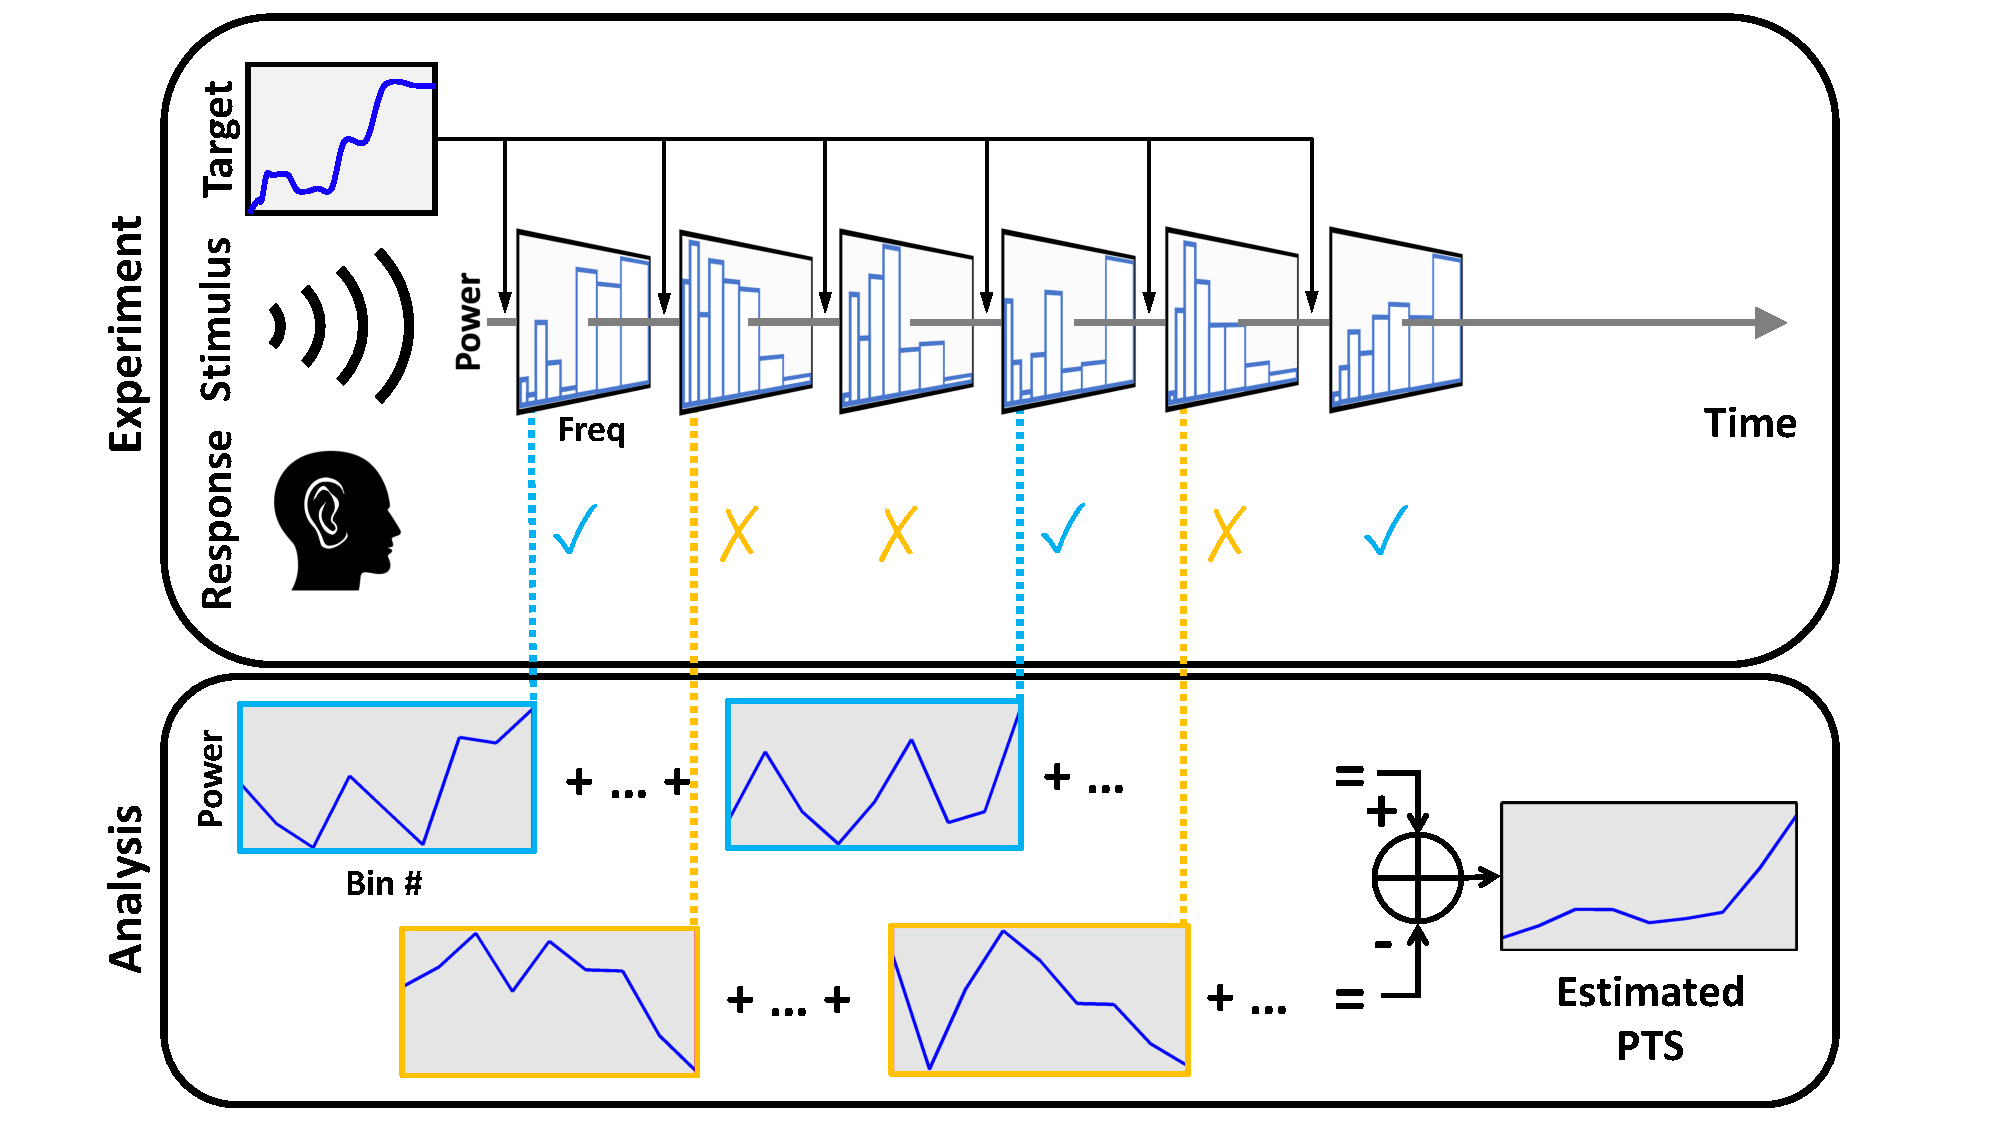
\includegraphics[width=\linewidth]{experiment_overview.pdf}
    \caption{Diagram of the experimental paradigm. The subject listens to a priming target signal,
  then a stimulus. They compare the mental model of the stimulus to the mental model of the target signal,
  before making a binary choice about the two signals' similarity.}
    \label{fig:experimentdiagram}
\end{figure}


% \subsection{Abbreviations and Acronyms}
% Define abbreviations and acronyms the first time they are used in the text, even after they have already been defined in the abstract. Abbreviations such as IEEE, SI, ac, and dc do not have to be defined. Abbreviations that incorporate periods should not have spaces: write “C.N.R.S.,” not “C. N. R. S.” Do not use abbreviations in the title unless they are unavoidable (for example, “IEEE” in the title of this article).

% needed in second column of first page if using \IEEEpubid
%\IEEEpubidadjcol


\section{Results}

% $n=10$ subjects performed an AX-paradigm reverse correlation experiment
% using two ATA tinnitus examples as the target sounds: 1``buzzing'' and ``roaring''.
% We reconstructed the PTS using the responses and stimuli from the experiments
% using $L_2$ linear regression.
% Additionally, we performed $n=1000$ \textit{in-silico} experiments
% using synthetic and random response algorithms.

Figure \ref{fig:reconstructions} reports Pearson's $r$ scores
for $n=10$ human, $n=1000$ synthetic, and $n=1000$ random subjects.
Most human subjects perform significantly better than the random baseline
and some approach the synthetic subject's empirical upper bound.
The distributions of human subject $r$ are significantly different
from the baseline random results (Mann-Whitney $U$ test, $p < 0.001$).
% $4$ subjects' results are statistically different from zero correlation
% ($p < 0.05$).

\begin{figure}[ht]
    \centering
    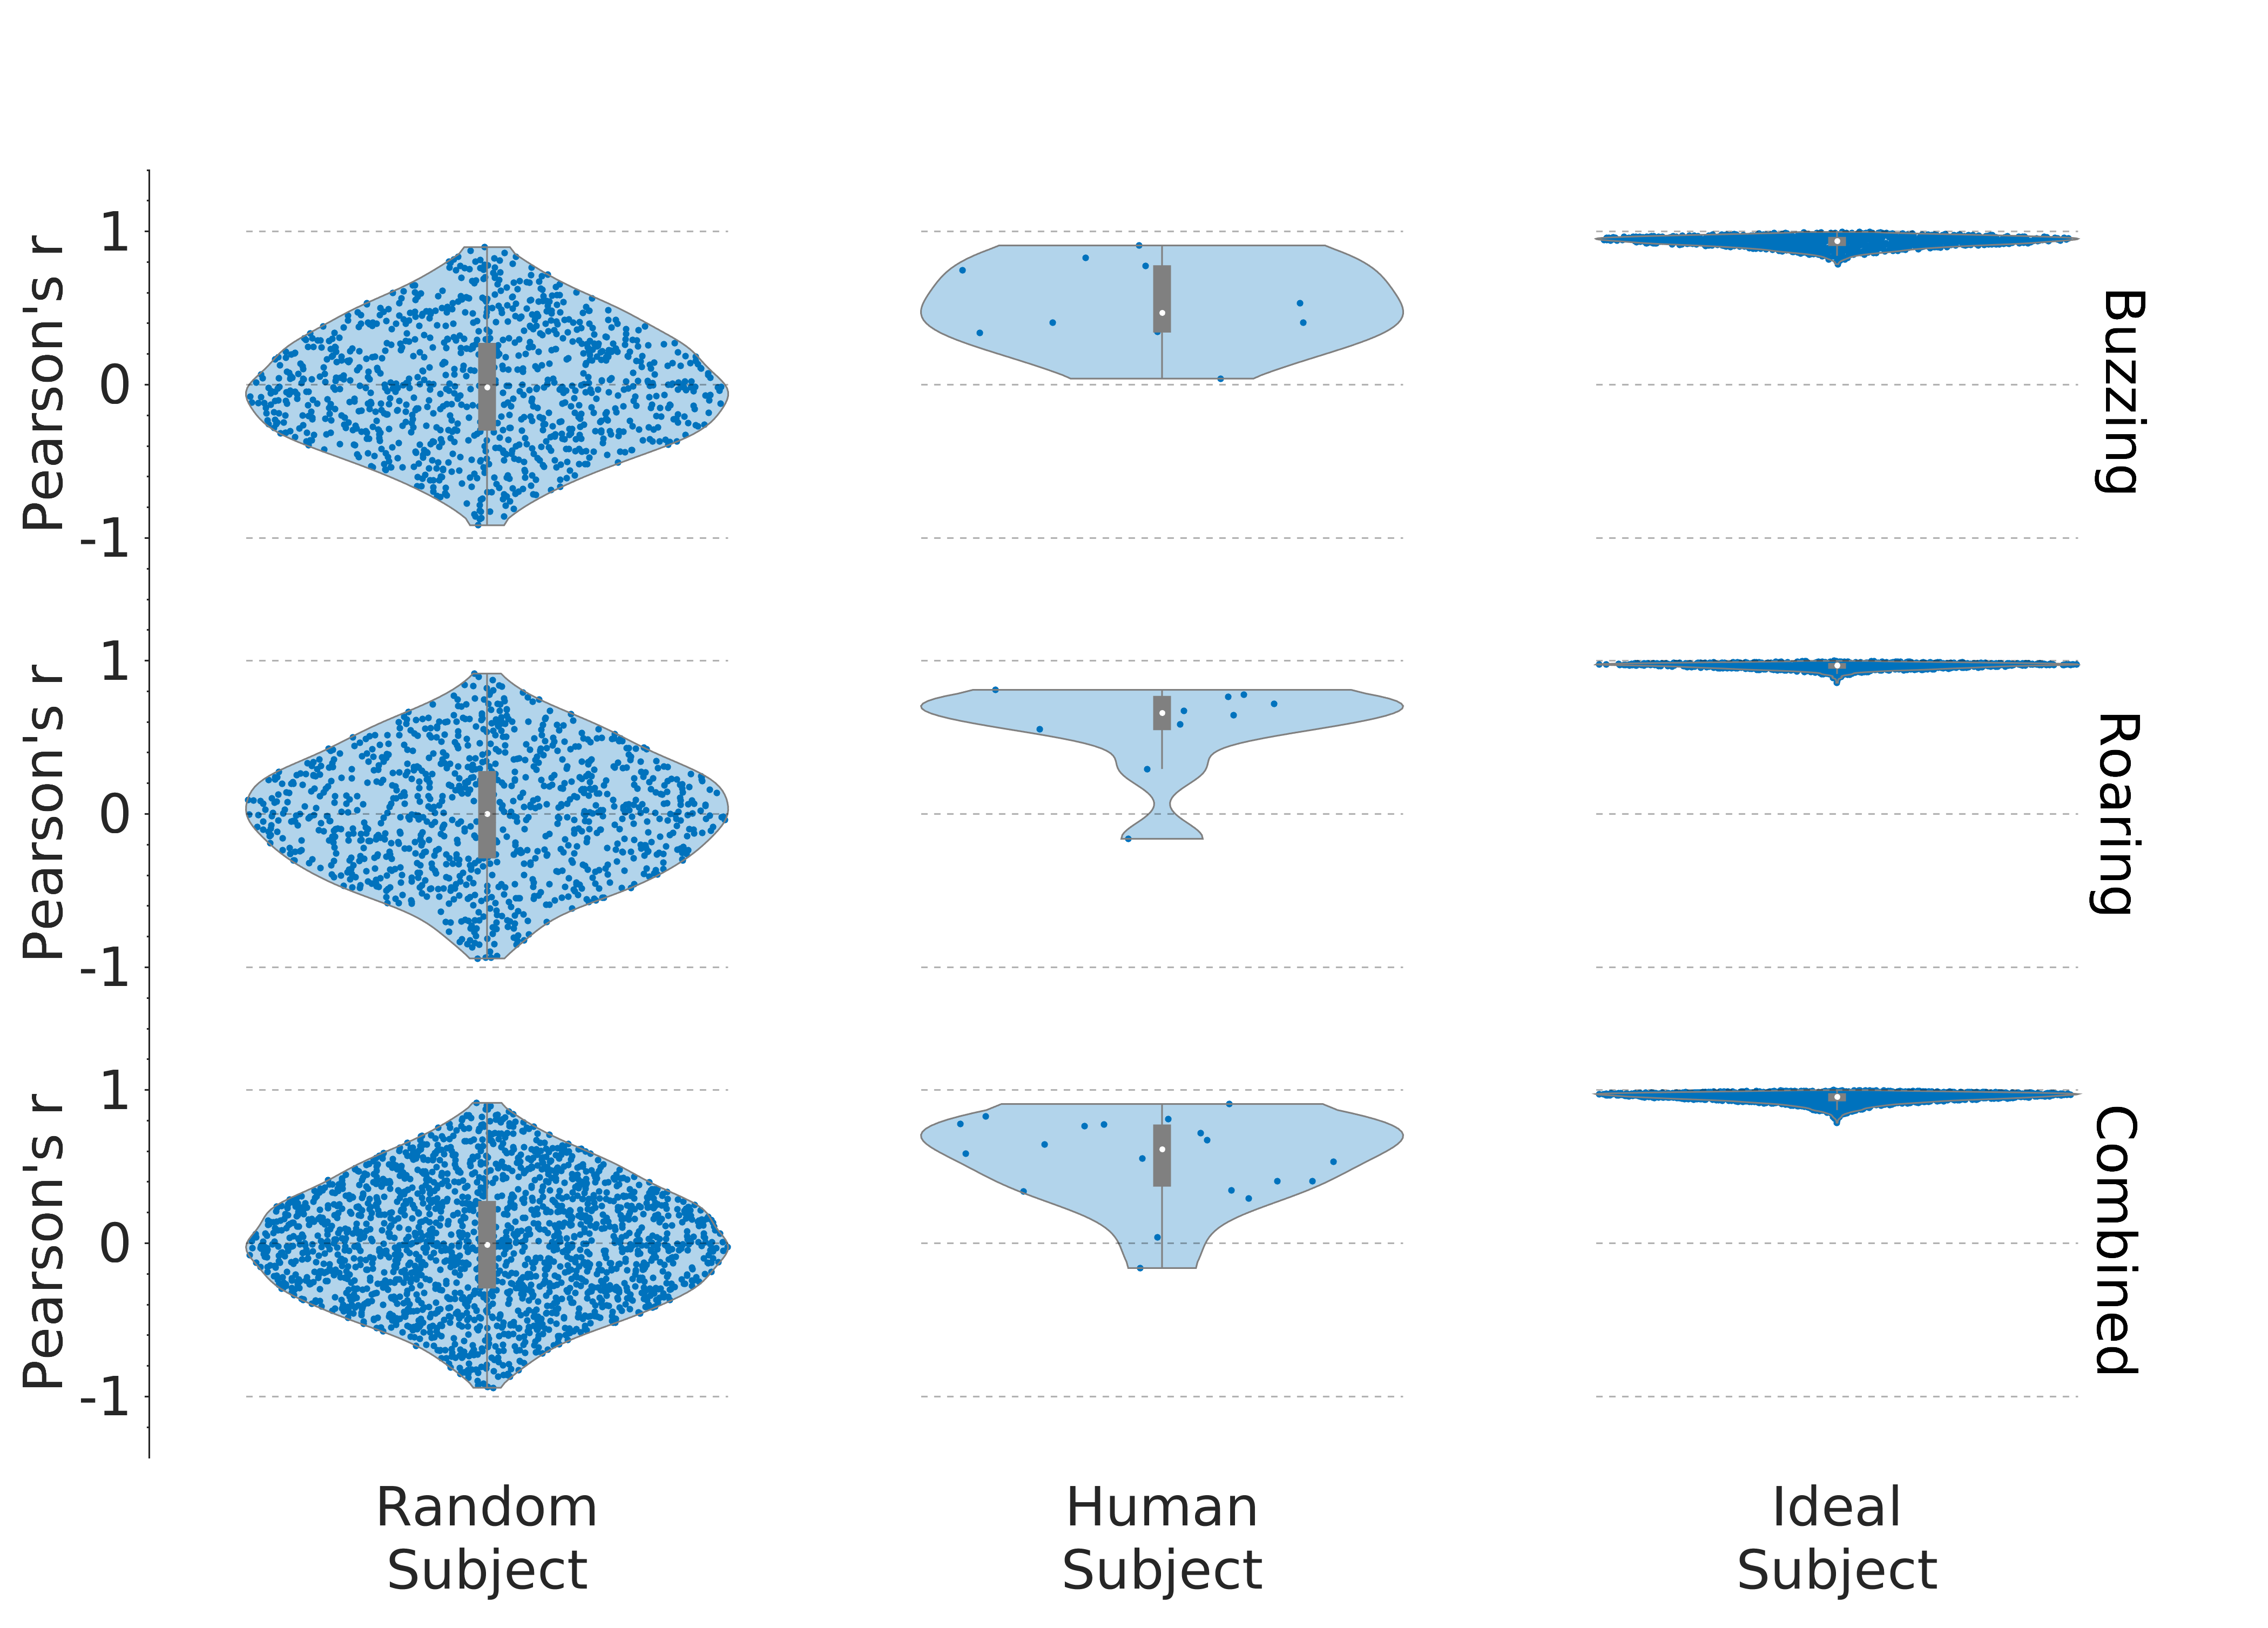
\includegraphics[width=\linewidth]{reconstruction_violin_1.eps}
    \caption{Reconstruction accuracy for human, synthetic, and random subjects,
    shown as violin plots with box plots overlaid. The median is a white dot,
    the ordinate of the blue points are the true Pearson's $r$ values \textemdash{}
    the abscissa has no meaning.
    \textbf{a-c} show violin plots for the buzzing target signal, 
    \textbf{d-f} show results the roaring target signal,
    and \textbf{g-i} show results for the all data combined.
    Human subjects perform significantly better than random chance
    and some approach the empirical maximum of the synthetic subject results
    (Mann-Whitney $U$ test, $p < 0.001$).}
    \label{fig:reconstructions}
\end{figure}

\begin{figure}[ht]
    \centering
    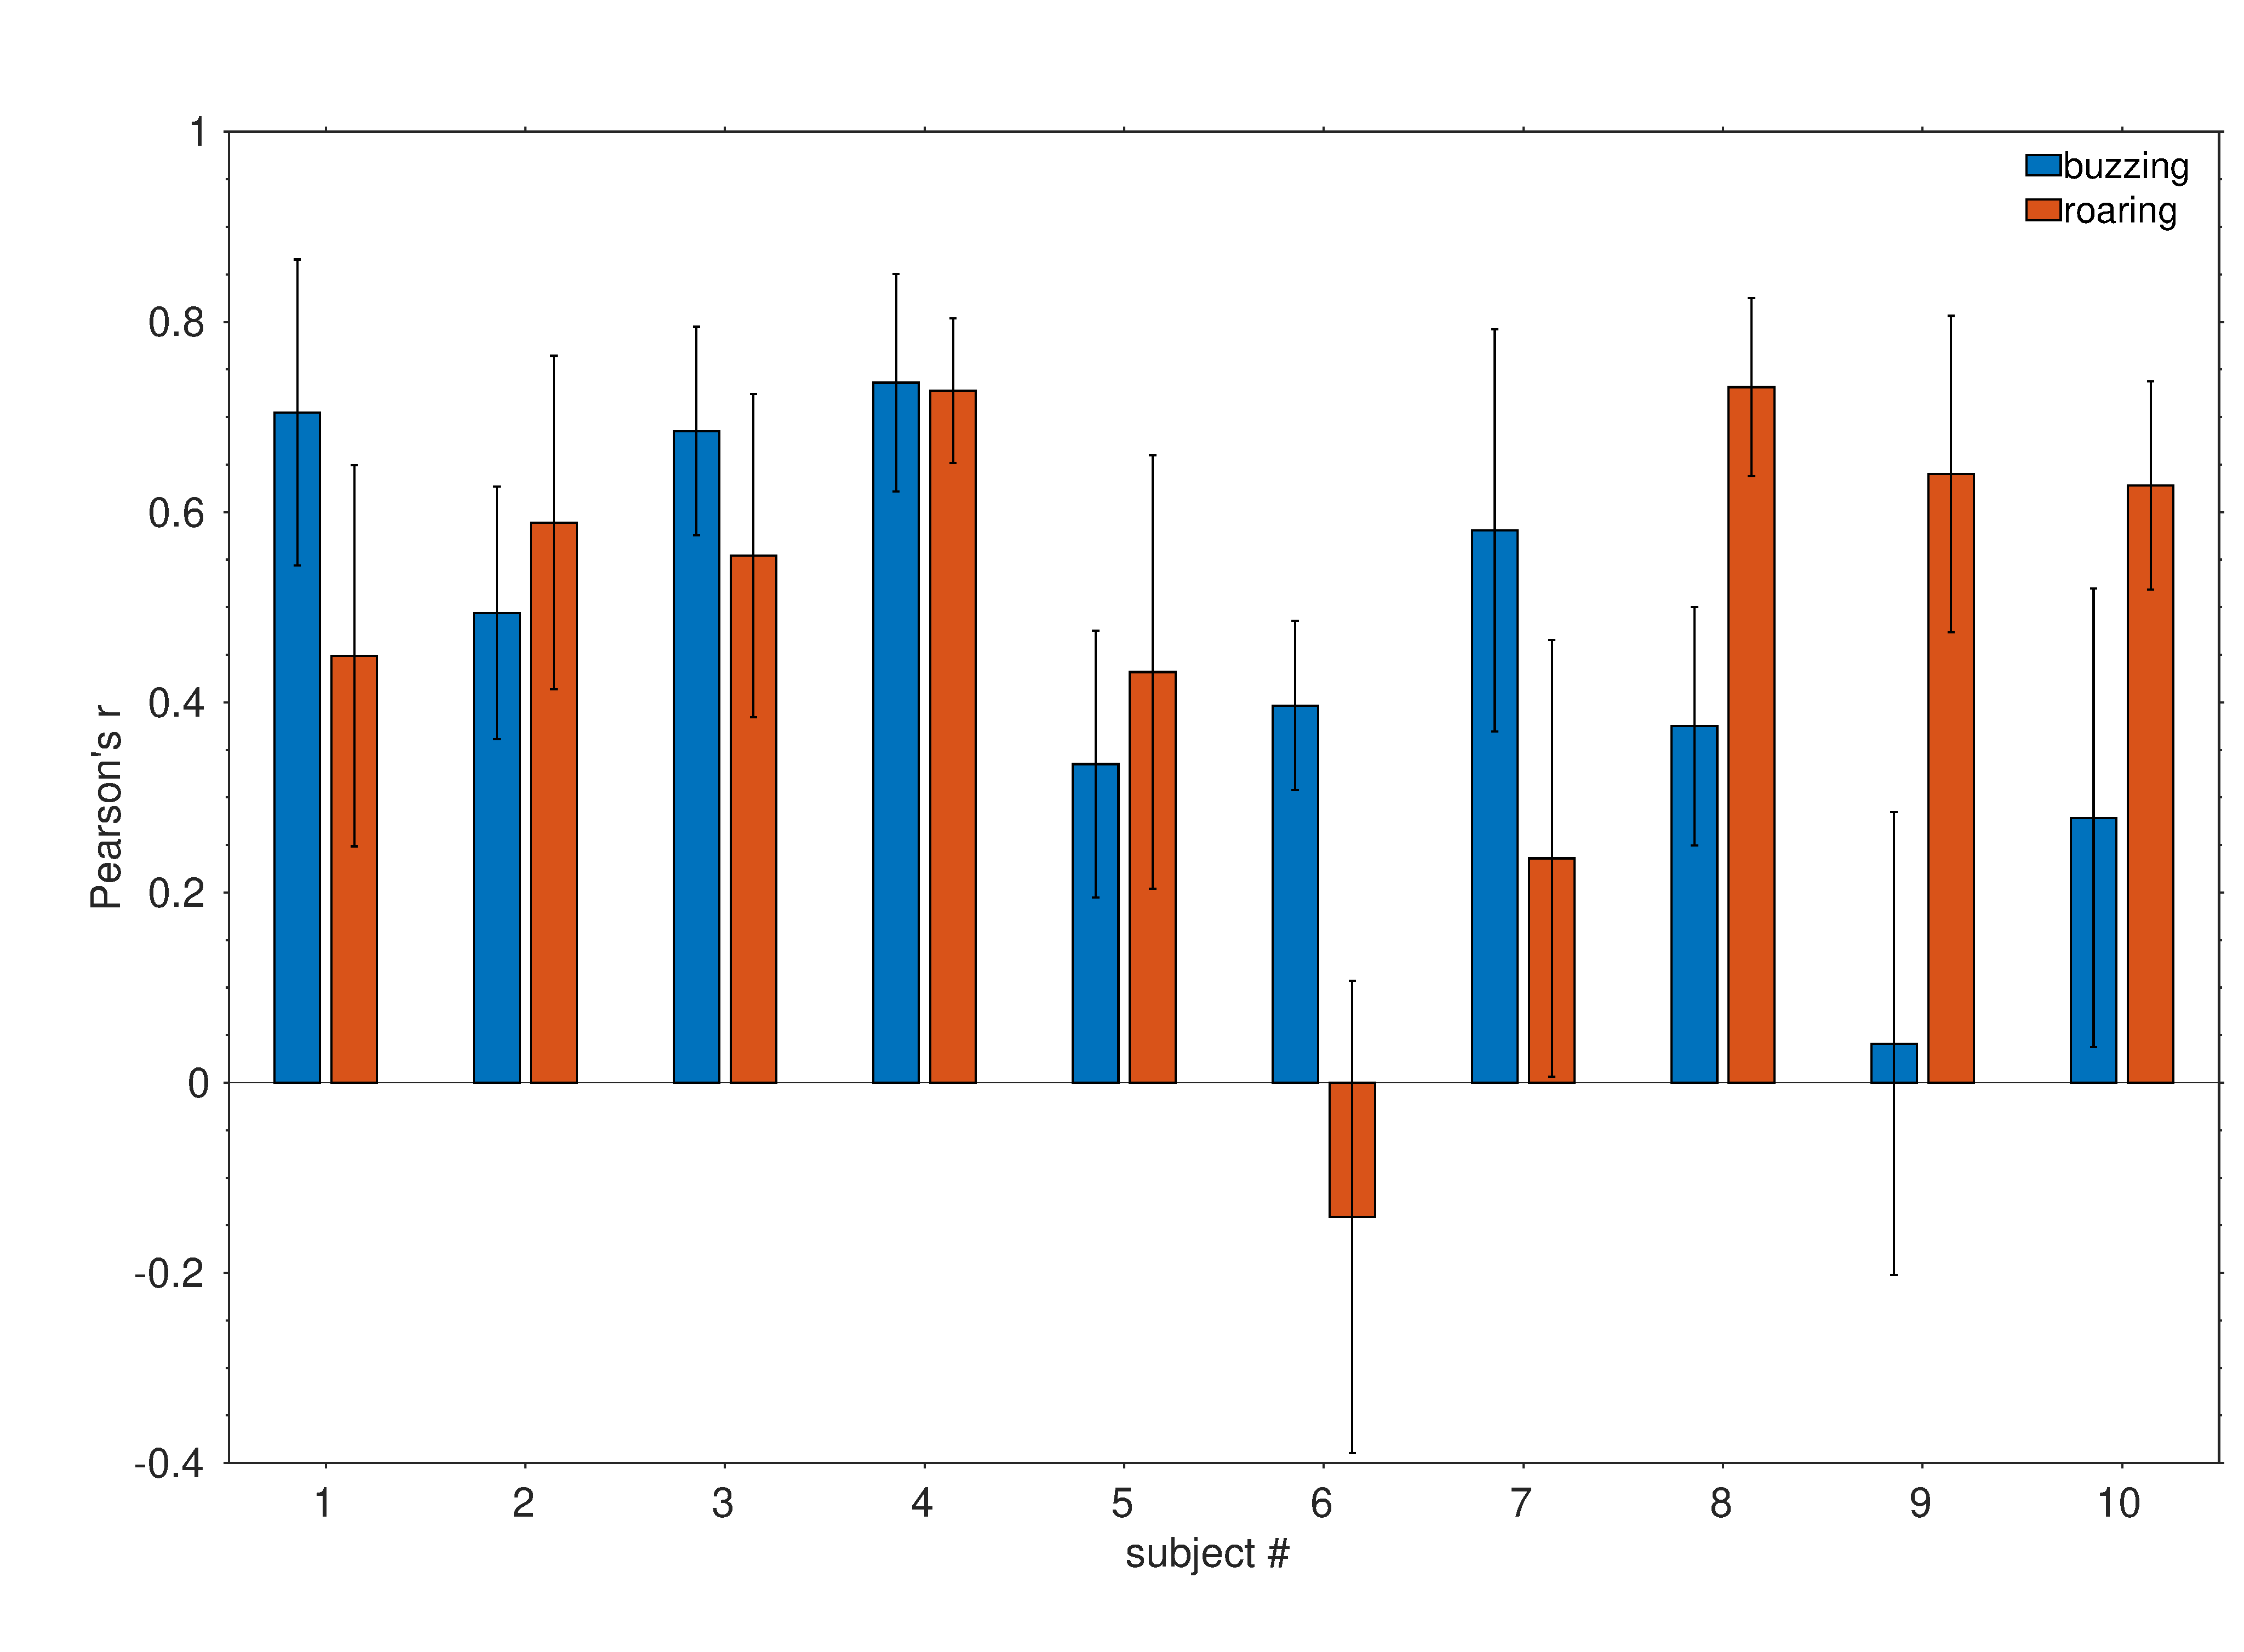
\includegraphics[width=\linewidth]{bootstrap_bar_errs.eps}
    \caption{aaa}
    \label{fig:bootstrapped}
\end{figure}

\section{To-Do}

\begin{enumerate}
    \item Follow-up results
    \item Results
    \item Conclusion
    \item Supplementary Info
    \item Abstract \& Visual Abstract
\end{enumerate}

\section{Conclusion}

We applied reverse correlation to the novel domain of psychoacoustic tinnitus spectrum reconstruction
and improved reconstruction performance (PTS) up to 2x using compressed sensing.
Using our reconstruction algorithm, the experiment required only 2,000 trials
for quality reconstruction results which is a 10x improvement over reverse correlation results in similar domains
\cite{gosselinSuperstitiousPerceptionsReveal2003}.
Subjects finished the experiment within two hours,
indicating that this procedure is feasible as an ``outpatient medical test''
to characterize the PTS of a subject,
a crucial step in diagnosis and treatment \cite{henryTinnitusEpidemiologicPerspective2020,henryMeasurementTinnitus2016,norenaPsychoacousticCharacterizationTinnitus2002}.
After fine-tuning, we will use this algorithm
to characterize the PTSes of clinical tinnitus patients
to help in the treatment of patients and to further understanding of tinnitus.

Results from human subjects are far below the synthetic baseline,
indicating that some improvements can be made to boost human performance.
The simplicity of the mathematical model for the synthetic subject
(and its favorability towards the problem)
leads to a synthetic subject that accounts for each tonotopic bin
with equal attentiveness, does not suffer fatigue, and never changes its
threshold for positive vs. negative responses.
The experiment asks subjects to rate each stimulus as 
similar or dissimilar to the target tinnitus signal.
This can lead to ``threshold drift,''
where the decision threshold between positive and negative assignments to stimuli
change as the experiment goes along.
While the AX paradigm protects against this effect somewhat
by playing the target sound before each decision stimulus,
subjects self-reported feeling unsure that they were making consistent decisions.
In future investigations,
we will use a two alternate forced choice (2AFC) paradigm,
where a subject is provided two stimuli after the cue,
and chooses the more similar one.
All chosen stimuli get positive responses assigned
and non-chosen stimuli get negative responses assigned (\hl{CITE?}).
Reconstructions can proceed normally, using both the positive and negative responses.

\hl{mention closed-loop/ML?}

% A conclusion section is required. Although a conclusion may review the main points of the paper, do not replicate the abstract as the conclusion. A conclusion might elaborate on the major findings and significance of the work or suggest applications and extensions. Do not exceed 300 words for the conclusion section.\\
% \\
% \textsc{Supplementary Materials}
% \par Supplementary materials are encouraged. Please use the Supplementary Materials template. If you have Supplementary Materials, please use this section to direct readers to the Supplementary Materials and give them a brief overview of what they can expect to find in the Supplementary Materials. \\
% \\
\textsc{Acknowledgment}
\par A. H. thanks Drs. Srinivas Gorur-Shandilya and Mark Zielinski for informative discussions regardining data visualization.
The authors thank Mr. Jacob Mills and Ms. Myah Caplan for their assistance in data collection. \\
% \\
% \textsc{REFERENCES AND FOOTNOTES}

% \subsection{References}

% See the end of this document for formats and examples of common references. For a complete discussion of references and their formats, see “The IEEE Style Manual,” available as a PDF link off the  \underline{\textit{Author Digital Toolbox}} main page.

% \subsection{Footnotes}
% Number footnotes separately in superscripts\footnote{It is recommended that footnotes be avoided (except for the unnumbered footnote with the receipt date on the first page). Instead, try to integrate the footnote information into the text.}.  Place the actual footnote at the bottom of the column in which it is cited; do not put footnotes in the reference list (endnotes). Use letters for table footnotes (see Table I). 



% \section{Submitting Your Paper for Review}

% {
% 	\subsection{Uploading the Document}
% 	All submissions must be uploaded via ScholarOne Manuscripts. Include full mailing addresses and e-mail addresses of all authors when uploading a manuscript. In addition, designate one author as the “corresponding author.” This is the author to whom proofs of the paper will be sent. Proofs are sent to the corresponding author only.
    
% 	\subsection{Review Stage Using ScholarOne$^{\tiny\textregistered}$ Manuscripts}
% 	Contributions to IEEE OJEMB must be submitted electronically on IEEE’s on-line manuscript submission and peer-review system, ScholarOne$^{\tiny\textregistered}$ Manuscripts at \textit{http://mc.manuscriptcentral.com/embs-ieee}. First check if you have an existing account. If there is none, please create a new account. After logging in, go to your Author Center and click “Submit First Draft of a New Manuscript.” 
% 	There are various steps to the submission process; you must complete all steps for a complete submission. At the end of each step you must click “Save and Continue”; just uploading the paper is not sufficient. After the last step, you should see a confirmation that the submission is complete. You should also receive an e-mail confirmation. For inquiries regarding the submission of your paper on ScholarOne Manuscripts, please contact oprs-support@ieee.org or call +1 732 465 5861.
    
% 	\subsection{Final Stage Using ScholarOne Manuscripts}
% 	Upon acceptance, you will receive an email with specific instructions regarding the submission of your final files.  To avoid any delays in publication, please be sure to follow these instructions.  Final submissions should include source files of your accepted manuscript, high quality graphic files, and a formatted pdf file.  If you have any questions regarding the final submission process, please contact the administrative contact for the journal. 
% }


% \section{Editorial Policy}
% {
% 	Do not publish “preliminary” data or results. The submitting author is responsible for obtaining agreement of all coauthors and any consent required from sponsors before submitting a paper. IEEE OJEMB strongly discourages courtesy authorship. It is the obligation of the authors to cite relevant prior work. IEEE OJEMB expects the main source of references be archival journal articles or books or thesis. Conference proceeding papers should be minimized since many are not undergoing rigorous peer reviews. 
% 	At least two reviews are required for every paper submitted. Indecipherable English is a valid reason for rejection. There is a service available that will help you improve your English for a fee, and the link to that service can be found at \textit{http://www.ieee.org/web/publications/authors/transjnl/ index.html}. 
    
% }

% \section{Publication Principles}
% {
% 	The two types of contents of that are published are; 1) peer-reviewed and 2) archival. IEEE OJEMB publishes scholarly articles of archival value as well as tutorial expositions and critical reviews of classical subjects and topics of current interest. 
% 	Authors should consider the following points:
% 	\begin{enumerate}
% 		\item Technical papers submitted for publication must advance the state of knowledge and must cite relevant prior work. 
% 		\item The length of a submitted paper should be commensurate with the importance, or appropriate to the complexity, of the work. 
% 		\item Authors must convince both peer reviewers and the editors of the scientific and technical merit of a paper; the standards of proof are higher when extraordinary or unexpected results are reported. 
% 		\item Because replication is required for scientific progress, papers submitted for publication must provide sufficient information to allow readers to perform similar experiments or calculations and use the reported results. Although not everything need be disclosed, a paper must contain new, useable, and fully described information. For example, a specimen’s chemical composition need not be reported if the main purpose of a paper is to introduce a new measurement technique. Authors should expect to be challenged by reviewers if the results are not supported by adequate data and critical details.
% 		\item Papers that describe ongoing work or announce the latest technical achievement, which are suitable for presentation at a professional conference, may not be appropriate for publication.
% 	\end{enumerate}
    
    
% }

\bibliographystyle{IEEEtran}
\bibliography{IEEEabrv,mybib}
% \printbibliography

% \begin{thebibliography}{1}
% 	%\textit{Basic Format for Books:}\\
% 	\bibitem{BasicBook} \textbf{Basic Format for Books:} J. K. Author, Title of chapter in the book, in \textit{Title of His Published Book}, xth ed. City of Publisher, Country if not USA: Abbrev. of Publisher, year, ch. x, sec. x, pp. xxx–xxx.
    
% 	\bibitem{ExampleBook1} \textit{Example Book 1:} G. O. Young, “Synthetic structure of industrial plastics”, in \textit{Plastics},  2nd  ed.,  vol.  3,  J.  Peters,  Ed.  New  York: McGraw-Hill, 1964, pp. 15–64.
    
% 	\bibitem{ExampleBook1} \textit{Example Book 2:} W.-K. Chen, \textit{Linear Networks and Systems}. Belmont, CA: Wadsworth, 1993, pp. 123–135.\\
    
% 	\bibitem{BasicPeriodical} \textbf{Basic Format for Periodicals:} J. K. Author, “Name of paper”, \textit{Abbrev. Title of Periodical},  vol. x, no. x, pp. xxx-xxx, Abbrev. Month, year.
    
% 	\bibitem{ExamplePeriodical1} \textit{Example Periodical 1:} J. U. Duncombe, “Infrared navigation—Part I: An assessment of feasibility”, \textit{IEEE Trans. Electron Devices}, vol. ED-11, no. 1, pp. 34–39, Jan. 1959.
    
% 	\bibitem{ExamplePeriodical2} \textit{Example Periodical 2:} E. P. Wigner, “Theory of traveling-wave optical laser”, \textit{Phys. Rev.}, vol. 134, pp. A635–A646, Dec. 1965.
    
% 	\bibitem{ExamplePeriodical3} \textit{Example Periodical 3:} E. H. Miller et al., “A note on reflector arrays”,\textit{ IEEE Trans. Antennas Propagat.}, to be published.\\
    
% 	\bibitem{BasicHandbook} \textbf{Basic Format for Handbooks:} \textit{Name of Manual/Handbook}, x ed., Abbrev. Name of Co., City of Co., Abbrev. State, year, pp. xxx-xxx.
    
% 	\bibitem{ExampleHandbook1} \textit{Example Handbook 1:} \textit{Transmission Systems for Communications}, 3rd ed., Western Electric Co., Winston-Salem, NC, 1985, pp. 44–60.
    
% 	\bibitem{ExampleHandbook2} \textit{Example Handbook 2:} \textit{Motorola Semiconductor Data Manual}, Motorola Semiconductor Products Inc., Phoenix, AZ, 1989.\\
    
% 	\bibitem{BasicBookOnline} \textbf{Basic Format for Books (when available online):} Author. (year, month day). \textit{Title}. (edition) [Type of medium]. volume (issue). Available: site/path/file
    
% 	\bibitem{ExampleBookOnline} \textit{Example Book Available Online 1:} J. Jones. (1991, May 10). \textit{Networks}. (2nd ed.) [Online]. Available: http://www.atm.com\\
    
% 	\bibitem{BasicJournalOnline} \textbf{Basic Format for Journals (when available online):} Author. (year, month). Title. \textit{Journal}. [Type of medium]. volume (issue), pages. Available: site/path/file 
    
% 	\bibitem{ExampleJournalOnline} \textit{Example Journal Available Online 1:} R. J. Vidmar. (1992,  Aug.).  On  the  use  of  atmospheric plasmas as electromagnetic reflectors. \textit{IEEE Trans. Plasma Sci.} [Online]. 21(3), pp. 876–880. Available: http://www.halcyon.com/pub/journals/21ps03-vidmar\\
    
% 	\bibitem{BasicConferenceOnline} \textbf{Basic Format for Papers Presented at Conferences(when available online):} Author. (year, month). Title. Presented at Conference title. [Type of Medium]. Available: site/path/file
    
% 	\bibitem{ExampleConferenceOnline} \textit{Example Conference Paper Available Online 1:} PROCESS  Corp.,  MA.  Intranets:  Internet  technologies deployed behind the firewall for corporate productivity. Presented at 
% 	INET96 Annual Meeting. [Online]. Available:  http://home.process.com/Intranets/wp2.htp\\
    
% 	\bibitem{BasicReportsOnline} \textbf{Basic Format for Reports and Handbooks (when available online):} Author.   (year,   month).   Title. Company . City, State or Country. [Type of Medium]. Available: site/path/file
    
% 	\bibitem{ExampleReportOnline} \textit{Example Report Available Online 1:}  S.L.Talleen. (1996, Apr.). The Intranet  Architecture:  Managing  information  in  the  new paradigm. Amdahl Corp., CA. [Online]. Available: http://www.amdahl.com/doc/products/bsg/intra/infra/html\\
    
% 	 \textbf{Basic Format for Computer Programs and Electronic Documents (when available online):} ISO recommends that capitalization follow the accepted practice for the language or script in which the information is given.
    
% 	\bibitem{ExampleProgramOnline}\textit{Example Program Available Online 1:} A. Harriman. (1993, June). Compendium of genealogical software. \textit{Humanist}. [Online]. Available e-mail: HUMANIST@NYVM.ORG Message: get GENEALOGY REPORT\\
    
% 	\bibitem{BasicPatentsOnline} \textbf{Basic Format for Patents (when available online):} Name of the invention, by inventor’s name. (year, month day). \textit{Patent Number} [Type of medium]. Available: site/path/file\\
    
% 	\bibitem{ExamplePatentOnline}\text{Example Patent Available Online 1:} Musical toothbrush with adjustable neck and mirror, by L.M.R. Brooks. (1992, May 19). \textit{Patent D326189} [Online]. Available: NEXIS Library: LEXPAT File: DESIGN
    
    
% \end{thebibliography}

% that's all folks
\end{document}


